% Varieties as Conditioning Structure - LVC Presentation
% Brett Reynolds
% March 13, 2026

\documentclass[aspectratio=169,14pt]{beamer}

% Theme
\usetheme{metropolis}
\usecolortheme{default}

% Fonts
\usepackage{fontspec}
\setmainfont{EB Garamond}
\setsansfont{Helvetica Neue}
\setmonofont{Menlo}

% Packages
\usepackage{booktabs}
\usepackage{tikz}
\usetikzlibrary{positioning,decorations.pathmorphing}

% Custom commands
\newcommand{\term}[1]{\textsc{#1}}
\newcommand{\mention}[1]{\textit{#1}}

% Remove navigation
\setbeamertemplate{navigation symbols}{}

% Metadata
\title{Varieties as Conditioning Structure}
\author{Brett Reynolds}
\institute{Humber College}
\date{LVC Research Group\\March 13, 2026}

\begin{document}

% ============================================================================
\begin{frame}
\titlepage
\end{frame}

% ============================================================================
\begin{frame}{}
\centering
\Large

With friends after school:\\[0.5em]
\textit{``Yo, mans made it---finally done that assignment.''}

\vspace{2em}
\pause

Ten minutes later, with a teacher:\\[0.5em]
\textit{``Yeah, I finished it this morning.''}

\end{frame}

% ============================================================================
\begin{frame}{}
\centering
\Large

What just happened?

\vspace{2em}
\pause

\begin{tabular}{rl}
Register shift? & \textit{(situation changed)}\\[0.5em]
\pause
Code-switching? & \textit{(between what and what?)}\\[0.5em]
\pause
Style-shifting? & \textit{(toward whose style?)}\\[0.5em]
\pause
Dialect suppression? & \textit{(is MTE a dialect?)}\\
\end{tabular}

\end{frame}

% ============================================================================
\begin{frame}{}
\centering
\Large

The standard labels don't quite fit.

\vspace{1em}

\normalsize
\textbf{Register} = situational variation\\
\textbf{Dialect} = geographic/social variation\\
\textbf{Discourse community} = group-based variation

\vspace{1em}
\pause

But these criteria blur and overlap.\\[0.5em]
What \textit{kind of thing} is the difference between \mention{mans} and \mention{I}?

\end{frame}

% ============================================================================
\begin{frame}{}
\centering
\Large

Different question:

\vspace{1em}

What makes a form \textbf{appropriate}---\\and what is that appropriateness \textbf{indexed to}?

\end{frame}

% ============================================================================
\begin{frame}{Two sources}

\textbf{Wiese (2023):} Grammar lives in \term{communicative situations}, not named languages. Varieties describe regularities across situations.

\vspace{1em}
\pause

\textbf{O'Connor (2019):} Linguistic choices solve \term{coordination problems}. What stabilises is what's useful, not what clusters naturally.

\vspace{1em}
\pause

\textbf{Combined:} Varieties are stable partitions of situation-space, shaped by coordination.

\end{frame}

% ============================================================================
\begin{frame}{}

\begin{center}
\Large
Appropriateness is indexed to \textbf{three different anchors}:
\end{center}

\vspace{1em}

\begin{center}
\large
\begin{tabular}{lll}
\toprule
\textbf{Anchor} & \textbf{Question} & \textbf{Old label}\\
\midrule
\textsc{Situation} & What's the context? & Register\\[0.4em]
\textsc{Ascription} & What are you treated as? & Dialect\\[0.4em]
\textsc{Identification} & Whose norms do you orient to? & Discourse community\\
\bottomrule
\end{tabular}
\end{center}

\end{frame}

% ============================================================================
\begin{frame}{}
\centering

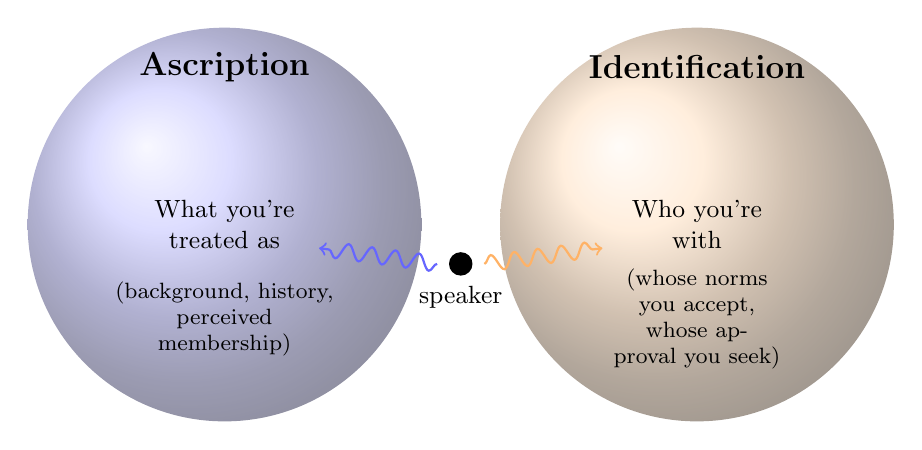
\begin{tikzpicture}
  % Left field - Ascription
  \shade[ball color=blue!30, opacity=0.6] (-3,0) circle (2.5cm);
  \node[font=\large\bfseries] at (-3,2) {Ascription};
  \node[font=\small, text width=3cm, align=center] at (-3,0) {What you're\\treated as};
  \node[font=\footnotesize, text width=3cm, align=center] at (-3,-1.2) {(background, history,\\perceived membership)};

  % Right field - Identification
  \shade[ball color=orange!30, opacity=0.6] (3,0) circle (2.5cm);
  \node[font=\large\bfseries] at (3,2) {Identification};
  \node[font=\small, text width=3cm, align=center] at (3,0) {Who you're\\with};
  \node[font=\footnotesize, text width=3cm, align=center] at (3,-1.2) {(whose norms you accept,\\whose approval you seek)};

  % Speaker in the middle
  \node[circle, fill=black, inner sep=3pt, label=below:{\small speaker}] at (0,-0.5) {};

  % Arrows showing pull
  \draw[->, thick, blue!60, decorate, decoration={snake, amplitude=1mm, segment length=3mm}] (-0.3,-0.5) -- (-1.8,-0.3);
  \draw[->, thick, orange!60, decorate, decoration={snake, amplitude=1mm, segment length=3mm}] (0.3,-0.5) -- (1.8,-0.3);
\end{tikzpicture}

\vspace{1em}
\pause

These can \textbf{align}---or they can \textbf{pull apart}.

\end{frame}

% ============================================================================
\begin{frame}{}
\centering
\Large

Back to our speaker.

\vspace{1.5em}

\normalsize
\begin{tabular}{ll}
\textbf{Ascription:} & MTE speaker (that's how they're heard)\\[1em]
\pause
\textbf{With friends:} & Identification aligns with ascription\\
& $\rightarrow$ \mention{mans made it}\\[1em]
\pause
\textbf{With teacher:} & Situation shifts---and maybe identification\\
& orients elsewhere\\
& $\rightarrow$ \mention{I finished it}\\
\end{tabular}

\end{frame}

% ============================================================================
\begin{frame}{}
\centering
\Large

Now imagine: years later, even with close friends,\\they say \mention{I} instead of \mention{mans}.

\vspace{1.5em}
\pause

The situation didn't change.\\[0.5em]
The ascription didn't change.\\[0.5em]
\pause
\textbf{The identification changed.}

\vspace{1.5em}
\pause

\textit{That's} where the agency is.

\end{frame}

% ============================================================================
\begin{frame}{}
\centering
\large

Style-shifting. Accommodation. ``Passing.''\\Professional socialisation. Code-switching.

\vspace{1.5em}

All of these live in the \textbf{gap}\\between ascription and identification.

\vspace{1.5em}
\pause

\normalsize
Not the only locus of agency---but a major one.

\end{frame}

% ============================================================================
\begin{frame}{}
\centering
\Large

Now the darker part.

\end{frame}

% ============================================================================
\begin{frame}{}
\centering
\large

A teacher hears \mention{mans} and something shifts---\\in their expectations, their evaluation, their behaviour.

\vspace{1.5em}
\pause

That shift is a \textbf{judgment of appropriateness},\\conditioned on an inferred ascription.

\vspace{1.5em}
\pause

And when everyone makes similar judgments,\\those judgments become \textbf{coordination signals}.

\vspace{1.5em}
\pause

\normalsize
``Standard'' vs ``non-standard'' = stable equilibrium.\\
Self-sustaining. Hard to exit unilaterally.

\end{frame}

% ============================================================================
\begin{frame}{}
\centering
\Large

This isn't an excuse. It's a diagnosis.

\vspace{1.5em}
\large

You can't talk your way out of a coordination problem.\\[0.5em]
\pause
The game structure has to change.

\end{frame}

% ============================================================================
\begin{frame}{}
\centering
\Large

So what changes?

\vspace{1.5em}
\pause

\normalsize
\textbf{For analysis:}\\
Register, dialect, discourse community\\aren't three kinds of thing.\\
They're three \textit{anchors} for appropriateness judgments.

\vspace{1em}
\pause

\textbf{For the phenomena:}\\
Watch the gap between ascription and identification.\\
That's where the action is.

\vspace{1em}
\pause

\textbf{For intervention:}\\
Change what's conditioned on, or change the consequences.

\end{frame}

% ============================================================================
\begin{frame}{}
\centering
\Large

\textbf{Discussion}

\vspace{1.5em}
\large

Does the ascription/identification distinction\\do useful work for what you study?

\vspace{1em}

How would you operationalise it?

\vspace{1em}

What breaks it?

\vspace{2em}
\small
Paper: \url{github.com/BrettRey/Varieties-as-Conditioning-Structure}

\end{frame}

\end{document}
